\chapter[Utilisation]{Utilisation}

\section{Lancement du programme}

Le lancement du programme se fait en lignes de commandes. Pour cela, il faut ouvrir un terminal dans le répertoire contenant le fichier python \textit{interface.py}. Le programme se lance lors de l'appel de ce fichier python : 
\begin{figure}[H]
	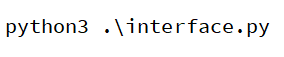
\includegraphics[scale=0.7]{lancement.png} 
	\label{fig:lancement}
\end{figure}

\section{Fonctionnement}

Lors de l'exécution du programme, une première fenêtre graphique s'ouvre.
\begin{figure}[H]
	\centering
	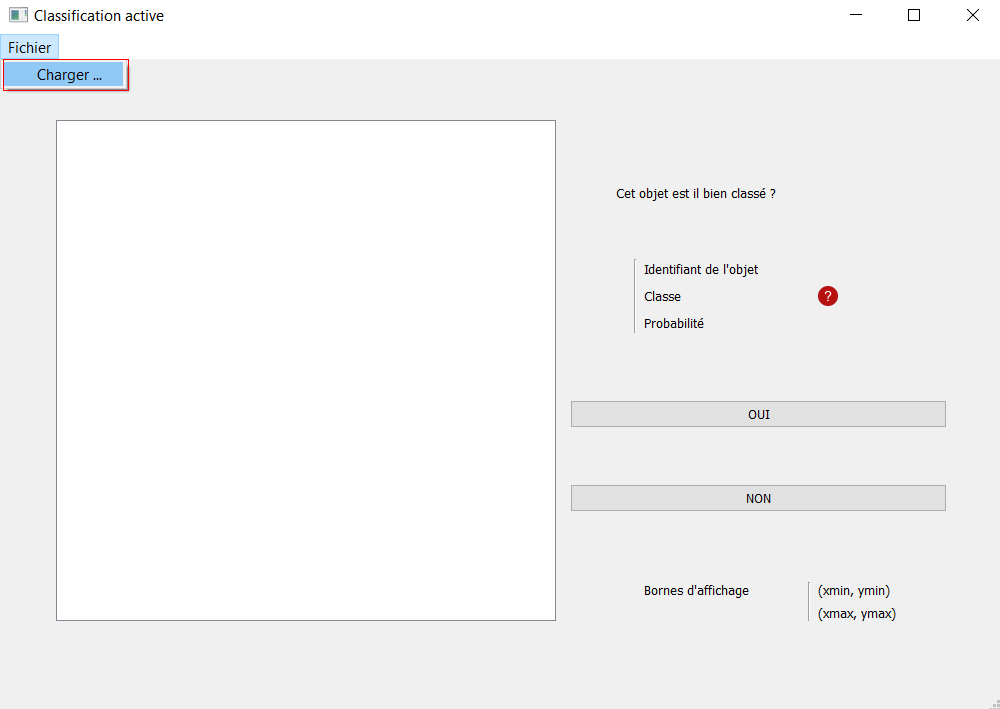
\includegraphics[scale=0.50]{1Charger.png} 
	\caption[Fenêtre principale]{Fenêtre principale}
	\label{fig:interfaceinitiale}
\end{figure}

La première étape consiste à charger les fichiers nécessaires au programme. Pour cela, il faut sélectionner le menu \textit{Fichier > Charger ...}. Une fenêtre de chargement s'ouvre.
\begin{figure}[H]
	\begin{minipage}{0.45\linewidth}
		\centering
		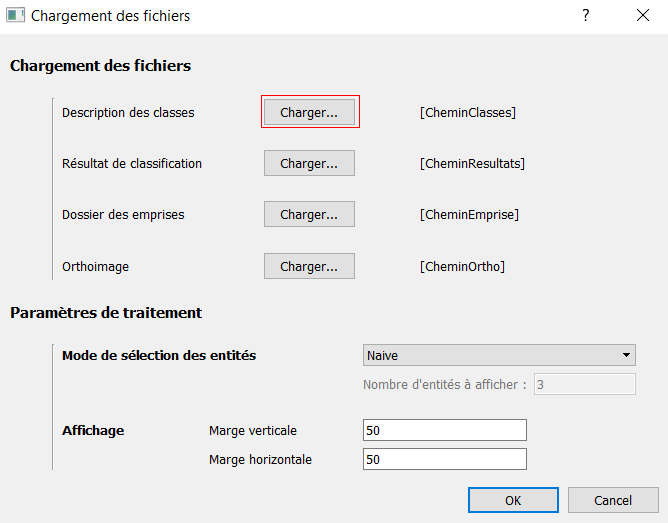
\includegraphics[scale=0.45]{2Charger1.png}  \\
	\end{minipage}
	\hfill
	\begin{minipage}{0.45\linewidth}
		\centering
		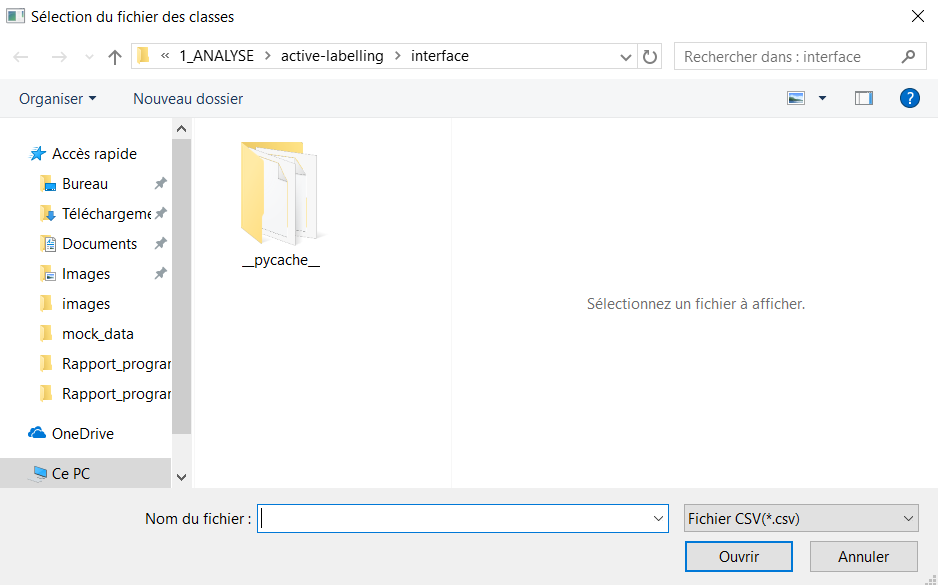
\includegraphics[scale=0.30]{2Charger2.png}  \\
	\end{minipage}
	\caption[Interface de chargement]{Interface de chargement}
	\label{fig:interfacecharger}
\end{figure}

Pour chaque fichier, sélectionner le chemin système correspondant. Une fois sélectionné, le chemin s'affiche dans l'interface. Avant de valider, deux paramètres de traitement doivent être renseignés : la méthode de sélection des entités à présenter et les valeurs des marges.\\

\begin{figure}[H]
	\centering
	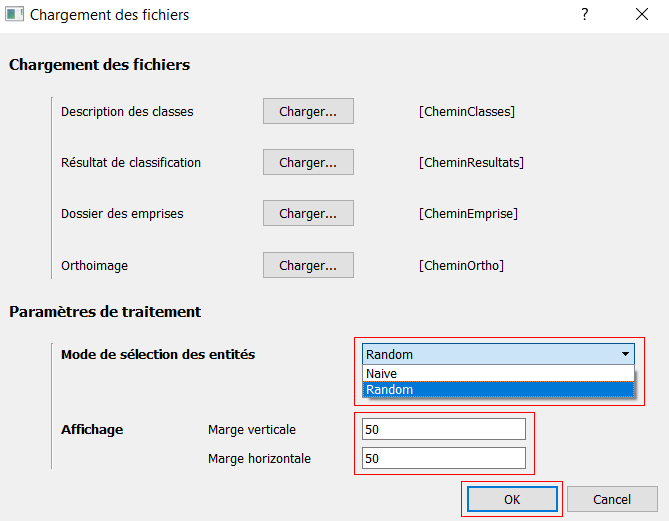
\includegraphics[scale=0.38]{3Param.png} 
	\caption[Choix des paramètres de traitement]{Choix des paramètres de traitement}
	\label{fig:paramtraitement}
\end{figure}

Lorsque tous les fichiers sont correctement chargés, et que les paramètres de traitement sont choisis, cliquer sur "OK". La visualisation des entités commence immédiatement. Pour chaque emprise visualisée, deux choix sont possibles : la validation ou l'invalidation de la classification. \\

\begin{figure}[H]
	\centering
	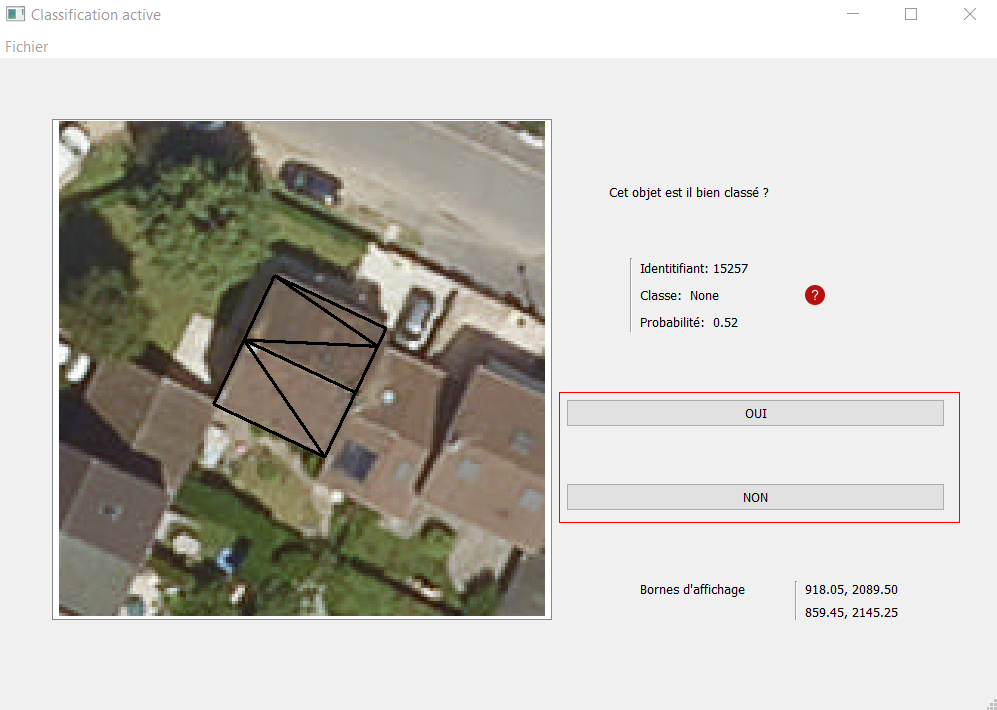
\includegraphics[scale=0.43]{4Valide.png} 
	\caption[Visualisation des entités et validation de la classification]{Visualisation des entités et validation de la classification}
	\label{fig:valide}
\end{figure}

En cas d'invalidation (si le bouton "NON" est cliqué), une seconde interface apparait et propose d'autres choix de classification. Une fois la nouvelle classe sélectionnée, valider le résultat en cliquant sur "OK".

\begin{figure}[H]
	\centering
	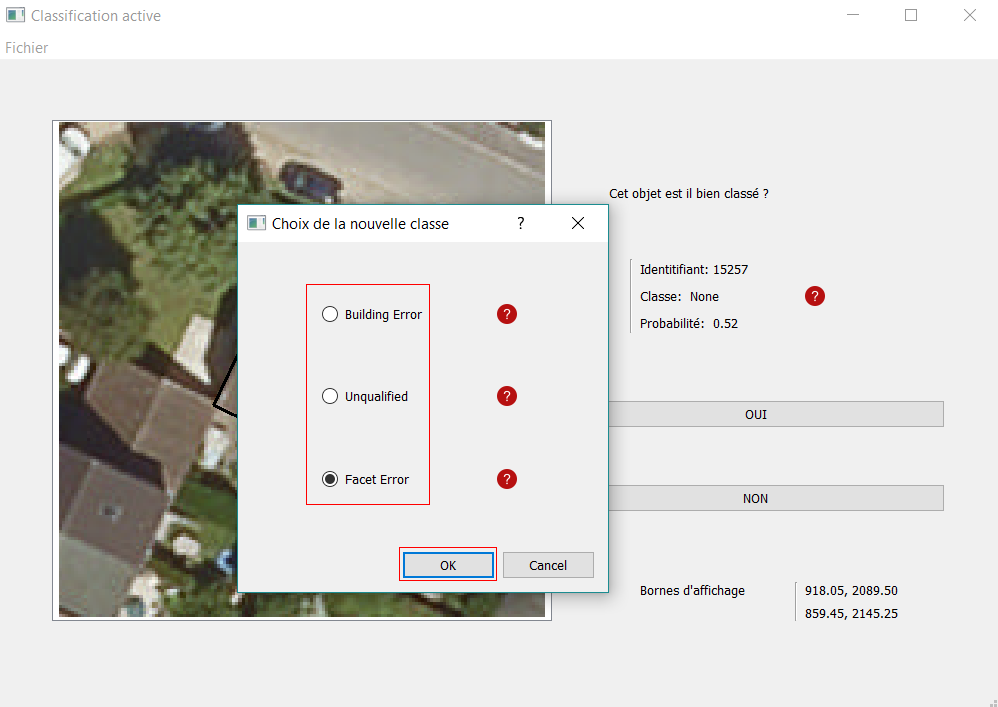
\includegraphics[scale=0.60]{5Select.png} 
	\caption[Visualisation des entités et validation de la classification]{Visualisation des entités et validation de la classification}
	\label{fig:valide}
\end{figure}

\begin{figure}[H]
	\begin{center}
		\begin{tabular}{m{.05\textwidth} m{.9\textwidth}}
			
\includegraphics[scale=0.20]{question.png} & En cas de doute sur la dénomination d'une classe, un survol de cette icône en affiche une brève description. \\
		\end{tabular}
	\end{center}
\end{figure}

Une fois la validation réalisée sur une entité, la suivante est directement affichée. Lorsqu'il n'y a plus d'emprise à afficher, une boite de dialogue s'ouvre, et permet de renseigner le chemin d'enregistrement du fichier des résultats.\\

\begin{figure}[H]
	\centering
	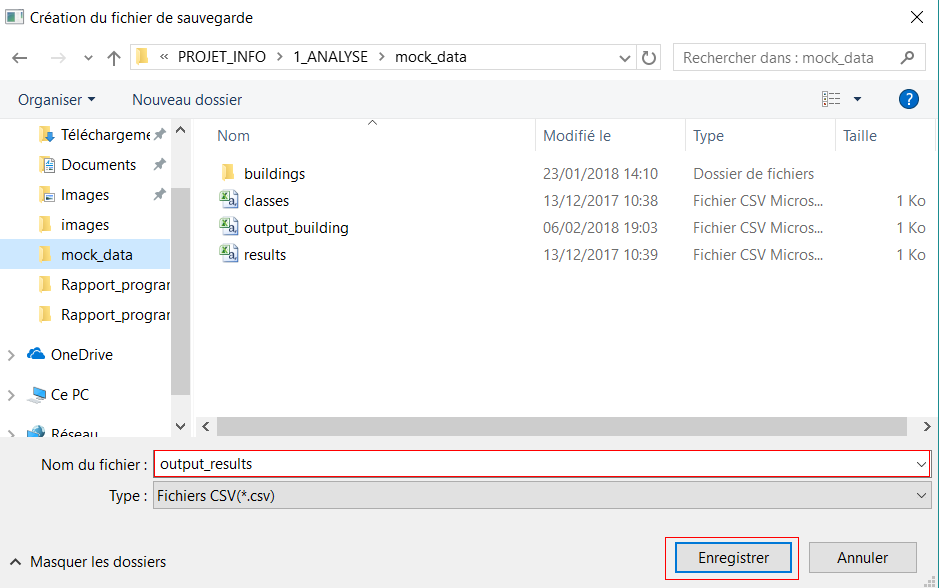
\includegraphics[scale=0.45]{6Save.png} 
	\caption[Enregistrement des résultats]{Enregistrement des résultats}
	\label{fig:save}
\end{figure}

Une fois le chemin validé, la validation est terminée et le programme se ferme.

\section{Données en sortie}

A l'issu du programme, un fichier .CSV est créé dans le répertoire choisi. Ce fichier a une structure identique aux résultats de l'auto-qualification donnés en entrée.

\begin{figure}[H]
	\centering
	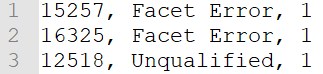
\includegraphics[scale=0.70]{7Results.png} 
	\caption[Exemple de fichier en sortie de traitement]{Exemple de fichier en sortie de traitement}
	\label{fig:outdata}
\end{figure}



